% Copyright (c) 2022 by Lars Spreng
% This work is licensed under the Creative Commons Attribution 4.0 International License. 
% To view a copy of this license, visit http://creativecommons.org/licenses/by/4.0/ or send a letter to Creative Commons, PO Box 1866, Mountain View, CA 94042, USA.

%~~~~~~~~~~~~~~~~~~~~~~~~~~~~~~~~~~~~~~~~~~~~~~~~~~~~~~~~~~~~~~~~~~~~~~~~~~~~~~
% You can add your packages and commands to the loadslides.tex file. 
% The files in the folder "styles" can be modified to change the layout and design of your slides.
% I have included examples on how to use the template below. 
% Some of these examples are taken from the Metropolis template.
%~~~~~~~~~~~~~~~~~~~~~~~~~~~~~~~~~~~~~~~~~~~~~~~~~~~~~~~~~~~~~~~~~~~~~~~~~~~~~~


\documentclass[
11pt,notheorems,hyperref={pdfauthor=whatever}
]{beamer}

\input{loadslides.tex} % Loads packages and some defined commands

\title[
% Text entered here will appear in the bottom middle
]{Ensemble learning}

\subtitle{How to use multiple times the same data}

\author[
% Text entered here will appear in the bottom left corner
]{
    Michele Vincenzo Branca, Leonardo De Pietro
}

\institute{
    Collegio Carlo Alberto, \\
    University of Turin}
\date{April 29, 2026}

% packages
\usepackage{amsmath}

\begin{document}

% Generate title page
{
\setbeamertemplate{footline}{} 
\begin{frame}
  \titlepage
\end{frame}
}
\addtocounter{framenumber}{-1}

\begin{frame}{Index of the presentation}
    % This stacks the sections from all three parts into one unified list
    \tableofcontents[part=1, hideallsubsections]
    \tableofcontents[part=2, hideallsubsections]
    \tableofcontents[part=3, hideallsubsections]
\end{frame}

\makepart{What is Ensemble Learning?}
\justifying
\section{What is Ensemble Learning?}
\subsection{An overview}
\begin{frame}
    Given a \emphasize{\textbf{supervised learning algorithm}} \(\mathcal{A}(\mathcal{D})\,:\,\mathcal{X}\to\mathcal{Y}\), can we run it more than once on datasets constructed from the original one \(\mathcal{D}\) and then (linearly!) combine the results to get an overall better predictor? Kind of.
    
    How do we do it for various algorithms?
    \begin{itemize}
        \item \alert{\textbf{local averaging methods}}: combine the predicted labels from estimators learned on different datasets;
        \item \alert{\textbf{regression}}: linearly combine the predictions;
        \item \alert{\textbf{classification}}: weighted majority vote or linear combination of real-valued predictions when convex surrogates are used.
    \end{itemize}
    What's the impact?
    \begin{itemize}
    \item for \example{\textbf{linear models}} this method does not add new functions, ;
    \item for \example{\textbf{non-linear models}} this method can add new functions. 
    \end{itemize}
    How do we construct the datasets? What are the benefits?
\end{frame}

\makepart{Averaging/Bagging}
\justifying
\section{Averaging}
\subsection{The framework}
\begin{frame}
    We will consider \alert{\textbf{regression with square loss}} where we have an explicit \example{\textbf{variance/bias}} decomposition.
    \begin{itemize}
        \item most results extend to other situations using convex surrogates.
    \end{itemize}

    \textbf{Setup:} \(m\) independent datasets of size \(n\), sampled \alert{\textbf{i.i.d.}} from \(p(x,\,y)\) distribution on \(\mathcal{X}\times\mathcal{Y}\). From each of them, we get an estimator \(\hat{f}^{(j)}\).

    \vspace{0.5em}
    \textbf{Averaged estimator:}
    \[
        \hat{f}^{\text{bag}}(x) = \frac{1}{m} \sum_{j=1}^m \hat{f}^{(j)}(x)
    \]

    \vspace{0.5em}
    \textbf{Impact on bias and variance}:
    \begin{itemize}
        \item \example{\textbf{bias}}: \(\text{bias}^{\text{bag}}(x) = \text{bias}^{(j)}(x)\), \(\forall\,j=1,\dots,\,m\);
        
        \item \example{\textbf{variance}}: \(\text{var}^{\text{bag}}(x) = \frac{1}{m}\text{var}^{(j)}(x)\).
    \end{itemize}

    \vspace{0.5em}
    \begin{block}{The ideal averaging effect}
        Because the datasets are strictly independent, averaging \(m\) models reduces the variance without introducing any additional bias.
    \end{block}
\end{frame}


\subsection{Example: \(k\)-nearest neighbor regression}

\begin{frame}
    \textbf{Expected excess risk bound under idealized averaging:}
    \[
        \int_{\mathcal{X}}\mathbb{E}\left[(\hat{f}(x)-f_\star(x))^2\right]\mathrm{d}p(x) \leq \underbrace{\frac{\sigma^2}{\textcolor{red}{m}k}}_{\text{variance bound}} + \underbrace{8B^2\text{diam}(\mathcal{X})^2\left(\frac{2k}{n}\right)^{2/d}}_{\text{bias bound}}
    \]
    This bound recovers the one for standard \(k\)-nearest neighbor when \(m=1\).\footnote{See Proposition 6.2, p. 170 \textit{Learning Theory from First Principles}, by \textit{Francis Bach}.}
    
    \vspace{0.5em}
    \textbf{Assumptions:} 
    \begin{itemize}
        \item \(\exists\,\sigma\geq0:(y-\mathbb{E}[y\mid x])^2\leq\sigma^2\) almost surely;
        \item \(f_\star\) \(B\)-Lipschitz-continuous;
        \item \(\text{diam}(\mathcal{X})<\infty\).
    \end{itemize}
    

    \vspace{0.5em}
    \textbf{Optimization and constraint on \(\boldsymbol{m}:\)}
    \begin{itemize}
        \item the \example{\textbf{optimal \(k\)}} balancing the bias-variance tradeoff is \(k \propto m^{-d/(2+d)} \cdot n^{2/(2+d)}\). The final risk scales as \(1/(mn)^{2/(2+d)}\), matching the rate of having a single massive dataset of \(N=nm\) observations!
        \item we need \(k>1\). Substituting in this condition the optimal \(k\), we see that \(m\) cannnot grow larger than \(n^{2/d}\).
    \end{itemize}
\end{frame}

\subsection{Example: ridge regression (misspecified model)}

\begin{frame}
    \textbf{Expected excess risk bound without averaging:}
    \[
        \begin{aligned}
            \int_{\mathcal{X}}\mathbb{E}\left[(\hat{f}(x)-f_\star(x))^2\right]\mathrm{d}p(x) &\leq \underbrace{\frac{\sigma^2}{n}\left(1+\frac{R^2}{\lambda n}\right)\text{tr}\left(\left(\Sigma+\lambda I\right)^{-1}\Sigma\right)}_{\text{variance upper bound}} + \underbrace{\left(1+\frac{R^2}{\lambda n}\right)^2\inf\limits_{f\in\mathcal{H}}\left\{\mid\mid f-f_\star\mid\mid^2_{L_2(p)}+\lambda\mid\mid f\mid\mid_{\mathcal{H}}^2\right\}}_{\text{bias upper bound}}\\
            & \propto \frac{\sigma^2}{n}\lambda^{-1/\alpha}+\lambda^{t/s}.
        \end{aligned}
    \]
    Averaging over \(m\) replications, the expected excess risk bound is proportional to: \(\frac{\sigma^2}{\textcolor{red}{m}n}\lambda^{-1/\alpha}+\lambda^{t/s}\).
    
    \vspace{0.25em}
    \textbf{Assumptions:}
    \begin{itemize}
        \item \(f_\star\in\) Sobolev Kernel of order \(t>0\);
        \item \(\mathcal{H}\) Sobolev space of order \(s>d/2\);
        \item \(\mid\mid\varphi(x)\mid\mid_\mathcal{H}\leq R\): A bounding constant for the feature norms.
        \item eigenvalues \((\lambda_m)\) of the covariance matrix \(\Sigma\) satisfy \(\lambda_m\leq C(m+1)^{\alpha}\), \(\alpha>1\).
    \end{itemize}  

    \vspace{0.5em}
    \textbf{Optimization:}
    \begin{itemize}
        \item exercise 10.2.
    \end{itemize}
\end{frame}


\section{Bagging}
\subsection{The framework}
\begin{frame}
    We will consider (again) \alert{\textbf{regression with square loss}} where we have an explicit \example{\textbf{variance/bias}} decomposition.
    \begin{itemize}
        \item most results extend to other situations using convex surrogates.
    \end{itemize}

    \textbf{Setup:} \(m\) datasets \(\mathcal{D}^{(b)}\), \(b=1,\dots,\,m\), each obtained with \alert{\textbf{random weights}} \(v_i^{(b)}\in\mathbb{R}_+\,i=1,\dots,n\)
    
    \vspace{0.5em}
    \textbf{Averaged estimator:}
    \[
        \hat{f}^{\text{bag}}(x) = \frac{1}{m} \sum_{j=1}^m \hat{f}^{(j)}(x)
    \]

    \vspace{0.5em}
    \textbf{Impact on Linear Estimators} (e.g., \example{kernel ridge}):
    \begin{itemize}
        \item \example{\textbf{bias:}} unchanged;
        \item \example{\textbf{variance:}} reduced.
    \end{itemize}

    \vspace{0.5em}
    \begin{block}{The bagging effect}
        Because bootstrap samples are drawn with replacement from the same original dataset, the models are correlated. Averaging them reduces the variance, but slightly increases the bias.
    \end{block}
\end{frame}


\subsection{Example: 1-nearest neighbor regression}
\begin{frame}
    In this case, the \textbf{bagged estimator} can be written as:
    \[
        \textcolor[gray]{0.65}{\frac{1}{m}\sum_{b=1}^m\hat{f}^{(b)}(x)=}\hat{f}(x) = \sum_{i=1}^n V_i y_{(i)}(x),
    \]
    where:
    \begin{itemize}
        \item \((x_{(i)}, y_{(i)})\) denotes the \(i\)-th closest neighbor to \(x\).
        \item \(V_i\) is the probability of remaining the \(i\)-th nearest neighbor in a (uniform) subsample of size \(s \geq 2\), independent from \(x\).
    \end{itemize}

    \vspace{0.5em}
    \textbf{Expected excess risk bound:}
    \[
        \int_{\mathcal{X}}\mathbb{E}\left[(\hat{f}(x)-f_\star(x))^2\right]\mathrm{d}p(x)\leq4B^2\text{diam}(\mathcal{X})^2\frac{1}{s^{2/d}}+\frac{s}{n}\frac{1}{(1+1/n-s/n)^2}.
    \]
    \textbf{Assumptions:}
    \begin{itemize}
        \item \(\exists\,\sigma\geq0:(y-\mathbb{E}[y\mid x])^2\leq\sigma^2\) almost surely;
        \item \(f_\star\) \(B\)-Lipschitz-continuous;
        \item \(\text{diam}(\mathcal{X})<\infty\).
    \end{itemize}

    \vspace{0.5em}
    \textbf{Optimization:}
    \begin{itemize}
        \item the \example{\textbf{optimal \(s\)}} balancing the bias-variance tradeoff is \(s^{1+2/d}\propto n\). This achieves the same performances as the \(k\)-nearest neighbor regression for a well-chosen \(k\).
    \end{itemize}
\end{frame}

\begin{frame}{}{Example: 1-nearest neighbor regression -- picture}
    \centering
    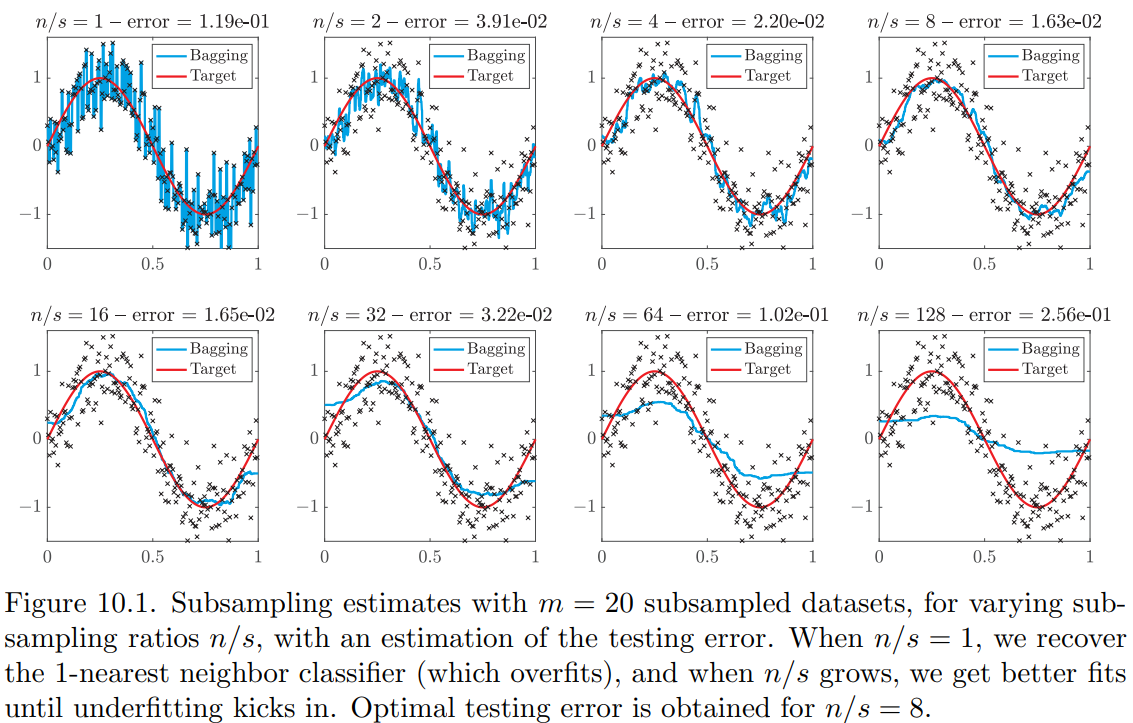
\includegraphics[width=0.8\textwidth]{img.png}
\end{frame}

\makepart{Random projections and averaging}
\justifying
\section{What are random projections?}
\subsection{An overview}

\begin{frame}
    Instead of reweighting observations, we can \alert{\textbf{randomly project}} the observations.

    \vspace*{0.5em}
    We will consider random projections for OLS (with the usual notation) in two settings:
    \begin{itemize}
        \item \alert{\textbf{sketching}}:
        \begin{itemize}
            \item the number of \example{\textbf{datapoints}} shrinks from \(n\) to \(s\). Typically, \(n > s > d\). This is an idealization of the subsampling of the previous part;
            \item practically, apply an i.i.d. Gaussian matrix \(S \in \mathbb{R}^{s \times n}\), going from \(\min_{\theta\in\mathbb{R}^d}\mid\mid y-\Phi\theta\mid\mid^2\) to \(\min_{\theta\in\mathbb{R}^d}\mid\mid Sy-S\Phi\theta\mid\mid^2\).
        \end{itemize}
        
        \vspace{0.25em}
        \item \alert{\textbf{random projection}}:
        \begin{itemize}
            \item the number of \example{\textbf{features}} shrinks from \(d\) to \(s\). Typically, \(d > n > s\);
            \item practically, apply a sketching matrix \(S \in \mathbb{R}^{d \times s}\), going from \(\min_{\theta\in\mathbb{R}^d}\mid\mid y-\Phi\theta\mid\mid^2\) to \(\min_{\eta\in\mathbb{R}^s}\mid\mid y-\Phi S\eta\mid\mid^2\).
        \end{itemize}
    \end{itemize}

    What's the impact?
    \begin{itemize}
        \item \example{\textbf{sketching}} reduced representation of data and computation time;
        \item \example{\textbf{random projection}} reduces computation time and \example{\textbf{regularizes}}.
    \end{itemize}
\end{frame}

\section{Gaussian sketching}
\subsection{Summary}
\begin{frame}
    \textbf{Sketched estimator:} 
    \(\hat{\theta} = \frac{1}{m} \sum_{j=1}^m \hat{\theta}^{(j)}\), where:
    \[
        \mathbb{R}^d\ni\hat{\theta}^{(j)} = (\Phi^\top(S^{(j)})^\top S^{(j)}\Phi)^{-1}\Phi^\top(S^{(j)})^\top S^{(j)}y,
    \]
    and \(S^{(j)} \in \mathbb{R}^{s \times n}\), \(j=1,\dots,\,m\).
    This provides an \alert{\textbf{unbiased}} estimator of the true OLS prediction: 
    \[
        \mathbb{E}[\Phi\hat{\theta}^{(j)}] = \Phi\hat{\theta}_{\text{OLS}}.
    \]

    \vspace{0.5em}
    \textbf{Expected generalization error:}
    \[
        \frac{1}{n} \mathbb{E}_{\varepsilon, S} \Bigg[ \bigg\| \frac{1}{m} \sum_{j=1}^m \Phi\hat{\theta}^{(j)} - \Phi\theta_* \bigg\|_2^2 \Bigg]=\underbrace{\frac{\sigma^2 d}{n}}_{\text{OLS baseline}} + \underbrace{\frac{\sigma^2 d}{mn}\left(\frac{n-d}{s-d-1}\right)}_{\text{algorithmic penalty}}.
    \]

    \vspace{0.5em}
    \textbf{Asymptotics and improvements:}
    \begin{itemize}
        \item \(m \to \infty\), the algorithmic penalty drops to zero and we recover the traditional OLS behavior;
        \item for \(m\) and \(s\) finite, the performance does not degrade too much;
        \item for \(m=s\) (even for \(m=1\)) we get twice the OLS performance;
        \item to get the same performance of OLS up to a factor of \(2\) we need \(m=(n-d)/(s-d-1)\sim n/s\) replications;
        \item again, there's no \example{\textbf{statistical gain}}, but rather a \example{\textbf{computational one}}.
    \end{itemize}
\end{frame}


\section{Random projections}
\subsection{Summary}
\begin{frame}
    We now assume \(d > n\), that is, an high-dimensional setup.
    \begin{itemize}
        \item OLS is \alert{ill-posed} because \(\Phi^\top\Phi\), whose rank is supposed to be \(n\), is not invertible.
    \end{itemize}

    A possible solution is:
    \begin{itemize}
        \item use a \alert{sketching matrix} \(S^{(j)} \in \mathbb{R}^{d \times s}\), with (\(s \le n\)) and \(j\in\{1,\dots,\,n\}\), sampled independently from an uknown distribution. Assume \(\text{rank}(S^{(j)}) = s\) a.s.;
        \item find the minimizer \(\hat{\eta}^{(j)}\) of \(\min_{\eta \in \mathbb{R}^s} \|y - \Phi S^{(j)}\eta\|_2^2\), assuming that \(\text{rank}(\Phi S^{(j)})=s\). Consider the average \(\hat{\theta}^{(j)} = S^{(j)}\hat{\eta}^{(j)}\);  
        \item consider the denoised resposnse vector is \(\hat{y}^{(j)} = \Pi^{(j)} y\), where \(\Pi^{(j)}\) is an \alert{orthogonal projection matrix} onto an \(s\)-dimensional vector space, such that, denoting its expectation \(\Delta = \mathbb{E}[\Pi^{(j)}]\), \(\text{tr}(\Delta) = s\).
    \end{itemize}
\end{frame}

\begin{frame}
    (Fixed design) \textbf{expected generalization error bound:}
    \[
        \frac{1}{n} \mathbb{E}_{\varepsilon, S} \left[ \bigg\| \frac{1}{m} \sum_{j=1}^m \hat{y}^{(j)} - \Phi\theta_* \bigg\|_2^2 \right] \le \frac{\sigma^2 s}{n} + \frac{1}{n} \theta_*^\top \Phi^\top \left[I - \Phi \mathbb{E}_S \big[SS^\top\big] \big( \mathbb{E}_S \big[SS^\top \Phi^\top \Phi SS^\top\big] \big)^{-1} \mathbb{E}_S \big[SS^\top\big] \Phi^\top\right]\Phi\theta_*,
    \]
    where the superscript \(^{(j)}\) has been omitted for clarity.

    \vspace{0.5em}
    Assuming \textbf{Gaussian random projections:} 
    \[
        \frac{1}{n} \mathbb{E}_{\varepsilon, S} \left[ \bigg\| \frac{1}{m} \sum_{j=1}^m \hat{y}^{(j)} - \Phi\theta_* \bigg\|_2^2 \right]\leq \underbrace{\frac{\sigma^2 s}{n}}_{\text{variance bound}} + \underbrace{\frac{2}{n}\text{tr}(\Phi^\top\Phi)\frac{\|\theta_*\|^2}{s+1}}_{\text{bias bound}}
    \]
    
    \vspace{0.25em}
    Note that this bound is of the form obtained for ridge regression with \(s\sim(\text{tr}(\Phi\Phi\top))/\lambda\).
\end{frame}

\subsection{Summary: sparse sketching matrixes}
\begin{frame}
    \textbf{Setup:} \(S \in \mathbb{R}^{d \times s}\) where each column is on of the \alert{\textbf{canonical basis vectors}} of \(\mathbb{R}^d\), \(e_i\), selected uniformly at random.

    \vspace{0.5em}
    \textbf{Expected generalization error bound:}
    \[
        \frac{1}{n} \mathbb{E}_{\varepsilon, S} \left[ \bigg\| \frac{1}{m} \sum_{j=1}^m \hat{y}^{(j)} - \Phi\theta_* \bigg\|_2^2 \right] \le \underbrace{\frac{\sigma^2 s}{n}}_{\text{variance bound}} + \underbrace{\frac{1}{n} \left( \frac{d}{s} \max_i(\|\phi_i\|_2^2) \|\theta_*\|^2 \right)}_{\text{bias bound}}
    \]

    \vspace{0.5em}
    \begin{block}{Comparison with what we had before:}
        \begin{itemize}
            \item the bias scales as \(\alert{d/s}\), not \(1/s\). We need \(s \propto d\) for a similar performance;
            \item the penalty source is governed by the \alert{maximum column norm} \(\max_i(\|\phi_i\|_2^2)\), rather than the full trace \(\text{tr}(\Phi^\top\Phi)\);
            \item computations are much faster because of sparsity, since we avoid costly matrix multiplications.
        \end{itemize}
    \end{block}
\end{frame}

\section{Kernel methods}
\subsection{Infinite-dimensional models and RKHS}
\begin{frame}
    \textbf{Setup:} instead of computing infinite-dimensional features \(\varphi(x) \in \mathcal{H}\), we access the space exclusively through the kernel: 
    \[ k(x, x') = \langle \varphi(x), \varphi(x') \rangle_{\mathcal{H}}. \]
    
    \vspace{0.25em}
    \textbf{Representer theorem:} 
    The infinite-dimensional risk minimization collapses into a finite span of the data: \(f(x) = \sum_{i=1}^n \alpha_i k(x, x_i)\).

    \vspace{0.5em}
    \begin{block}{The Matrix Algebra Swap}
        \begin{itemize}
            \item \alert{\textbf{the problem:}} standard models need the \(d \times d\) covariance matrix \(\Phi^\top\Phi\). Intractable if \(d = \infty\);
            \item \example{\textbf{the dual solution:}} we use the computable \(n \times n\) Kernel matrix \(K = \Phi\Phi^\top\);
            \item \example{\textbf{the parameter shift:}} we model \(y_* = K\alpha\) and solve for \(n\) scalar weights (\(\alpha\)) instead of \(\infty\) parameters (\(\theta_*\)).
        \end{itemize}
    \end{block}
\end{frame}

\begin{frame}
    \textbf{The bottleneck:} 
    finding weights \(\alpha = (K + \lambda I_n)^{-1}y\) requires inverting an \(n \times n\) matrix, taking \alert{\textbf{\(\mathcal{O}(n^3)\)}} time.

    \vspace{0.5em}
    \textbf{The sketching idea:} 
    use a sketch \(\hat{\Phi} \in \mathbb{R}^{n \times s}\) drawn from \(\mathcal{N}(0, K)\). This drops the inversion cost to \(\mathcal{O}(s^3)\), yielding:
    \[
        \text{Risk} \le \underbrace{\frac{\sigma^2 s}{n}}_{\text{variance bound}} + \underbrace{\frac{2}{n}\text{tr}(K)\frac{y_*^\top K^{-1} y_*}{s+1}}_{\text{bias bound}}
    \]

    \vspace{0.5em}
    \begin{block}{\emphasize{The \(\mathcal{O}(n^3)\) catch}}
        Sampling from \(\mathcal{N}(0, K)\) requires computing the matrix square root \(K^{1/2}\), which \textit{also} takes \alert{\textbf{\(\mathcal{O}(n^3)\)}} time. This exact sketching method is computationally useless!
    \end{block}
\end{frame}

\subsection{Random Fourier Features (RFF)}

\begin{frame}
    \alert{\textbf{The goal:}} build the \(n \times s\) sketch matrix \(\hat{\Phi}\) \textit{without} ever computing the \(n \times n\) Kernel matrix \(K\).

    \vspace{0.5em}
    \textbf{The trick (Bochner's theorem):} 
    translation-invariant kernels can be rewritten as an expected value over random frequencies \(v\):
    \[
        k(x, x') = \mathbb{E}_v \big[ \varphi(x, v)\varphi(x', v) \big].
    \]

    \vspace{0.25em}
    \textbf{The RFF algorithm:}
    approximate the expectation by sampling \(s\) random frequencies \(v_1, \dots, v_s\). We construct \(\hat{\Phi}\) directly. Each column \(j\) is just our data evaluated at one random frequency: \(\big(\varphi(x_1, v_j), \dots, \varphi(x_n, v_j)\big)^\top\)\footnote{Rahimi and Recht, 2008 propose the use of \(\varphi(x, v) = \sqrt{2}cos(v^\top x + b)\) with $b$ sampled uniformly in $[0, 2\pi]$}.
    \vspace{0.5em}
    \begin{block}{\example{The Ultimate payoff}}
        By completely bypassing \(K\), we drastically reduce our complexity:
        \begin{itemize}
            \item \textbf{Time to build sketch \(\hat{\Phi}\):} \(\mathcal{O}(ns)\)
            \item \textbf{Time to solve OLS:} \(\mathcal{O}(ns^2)\)
        \end{itemize}
    \end{block}
\end{frame}

\subsection{The Johnson-Lindenstrauss Lemma}
\begin{frame}
    Why do random projections work so well geometrically? 
    
    The \alert{\textbf{Johnson-Lindenstrauss lemma}} states that given \(\varphi_1,...,\varphi_n\;\in \mathbb{R}^d\), let \(S \in \mathbb{R}^{d \times s}\) be a random matrix with independent standard Gaussian variables. Then, for any \(\epsilon \in (0, 1/2)\) and \(\delta \in (0, 1)\), if \(s \ge \frac{6}{\varepsilon^2} \log \frac{n^2}{\delta}\), with probability greater than \(1-\delta\), we have
    \[
        \forall i,j \in \{1,...,n\}\;(1-\varepsilon)\|\varphi_i - \varphi_j\|_2^2 \le \|s^{-1/2}S^\top \varphi_i - s^{-1/2}S^\top \varphi_j\|_2^2 \le (1+\varepsilon)\|\varphi_i - \varphi_j\|_2^2
    \]
    Crucially, the required projected dimension \(s\) depends \example{\textbf{only logarithmically on \(n\)}} and is completely independent of the original dimension \(d\).
\end{frame}


\end{document}
